\documentclass[12pt, openany]{report}

\input{styles.tex}

\begin{document}
\selectlanguage{french}
% Édite style sous-titre image et tableau
\makeatletter
\newcommand{\figcapfont}{\itshape} 
\newcommand{\tabcapfont}{\itshape}
\renewcommand{\fnum@figure}{\figcapfont Image \thefigure}
\renewcommand{\fnum@table}{\tabcapfont Tableau \thetable}
\makeatother

\begin{titlepage}
  \begin{center}

    % Logo Esir and Irisa
    % Author and supervisor
    \begin{minipage}{0.45\textwidth}
      \begin{flushleft} \large
        \includegraphics[width=0.9\columnwidth]{datas/logo_esir.jpg}~\\
        \emph{Élève-ingénieur :}\\
        Tugdual Le Pen\\
        Imagerie Numérique\\
        3\up{ème} année du cursus ingénieur\\
        ~\\~\\
        \emph{Tuteur universitaire :}\\
        Pierre Maurel\\
        Enseignant Chercheur
      \end{flushleft}
    \end{minipage}
    \begin{minipage}{0.45\textwidth}
      \begin{flushright} \large
        \vspace{34pt}
        \includegraphics[width=0.9\columnwidth]{datas/logo_bcom.jpg}~\\
        \vspace{29pt}
        b<>com\\
        ZAC des Champs Blancs\\
        1219 avenue Champs Blancs\\
        35510 Cesson-Sévigné\\
        02 56 35 88 00\\
        ~\\
        \emph{Tuteur d'entreprise :}\\
        Duong Nam Duong\\
        Ingénieur b<>com\\
      \end{flushright}
    \end{minipage}

    \vspace{4cm}

    \textsc{\Huge \textbf{Reconstruction dense d'un modèle 3D à partie d'images RGB}}\\    
    \comment{Work in progress}
    \vfill

    % Bottom of the page
    \begin{minipage}{0.45\textwidth}
      \begin{flushleft}
        \vspace{0.5cm}
        {\large Année universitaire 2020 - 2021}
      \end{flushleft}
    \end{minipage}
    \begin{minipage}{0.45\textwidth}
      \begin{flushright}
        \includegraphics[width=0.9\columnwidth]{datas/logo_univ.png}~\\
      \end{flushright}
    \end{minipage}

  \end{center}
\end{titlepage}

% Actualise le compteur de page
\clearpage
\setcounter{page}{2}

% \include{chapter/remerciements}

\addcontentsline{toc}{chapter}{Résumé}
\chapter*{Résumé}


\vspace{40pt}

\selectlanguage{english}
\color{gray}



\selectlanguage{french}
\color{black}

% Renomme "Tables des matières" en "Sommaire"
\renewcommand{\contentsname}{Sommaire}
{\setlength{\parskip}{6pt}
\tableofcontents
}

\chapter{Introduction}

\par
\textbf{Rapide contexte}

\par
\textbf{Intro photogramétrie, env3D et réalité virtuelle}

\par
\textbf{Intro entreprise et équipe IMT}

\par
\textbf{Explication sujet de stage}

\par
\textbf{Explication trouver le stage et motivation pour le stage}



\chapter{Présentation de b<>com}

\par
Depuis sa création en 2012, l'Institut de Recherche Technologie b<>com a pour but de développer des technologies numériques ayant pour objectif d'améliorer la compétitivité des entreprises partenaires.

\par
C'est aujourd'hui ..

\chapter{Contexte}

\par
Environnements 3D et réalité virtuelle

\section{Photogramétrie}

\par
Définition

\par
Structure from Motion (SFM)

\par
Simultaneus Localisation and Mapping (SLAM)

\par
Multi-View Stereo (MVS)

\section{Framework SolAR}

Introduction et definition du framework

\addimage{logo_solar.png}{Logo de SolAR}

Explication du fonctionnement de SolAR

Présentation de l'équipe autour de SolAR

Pourquoi le besoin d'ajouter SFM et MVS



\chapter{Etat de l'art}
\par
La première étape de mon stage consiste à créer un module de reconstruction 3D dans le framework SolAR. Ce module est très complexe et demanderait énormément de travail et de temps pour pouvoir être créer à partir de zéro. On va donc chercher un logiciel sous licence libre afin de pouvoir l'utiliser et/ou le modifier si besoin. Afin de trouver le logiciel le plus adapté à notre utilisation, on va faire un état de l'art de différents logiciels de reconstruction 3D. 

\section{Préparatifs}

% Présentation des datasets utilisés (nb images, taille image, insideout/outside in)
Afin de pouvoir tester les différents programme de l'état de l'art, il nous faut des datasets d'images. J'en ai selectionné deux avec des caractéristiques différentes : \emph{Dinosaure} et \emph{Museum} (voir image \ref{fig:dataset_exemple}). 

\begin{figure}[ht]
    \centering
    \begin{subfigure}{0.40\textwidth}
        \includegraphics[width=\linewidth]{datas/dino_image.jpg}
        \caption{}
    \end{subfigure}
    \begin{subfigure}{0.47\textwidth}
        \includegraphics[width=\linewidth]{datas/museum_image.jpg}
        \caption{}
    \end{subfigure}

    \caption{Extrait du dataset \emph{Dinosaure} (a) et du dataset \emph{Museum} (b)}
    \label{fig:dataset_exemple}
\end{figure}

Le premier, une statuette de dinausaure, est composé de 53 images avec une résolution de 4912 x 3264. Celui-ci est assez léger en terme de nombre d'image est est qualifié de \emph{outside-in}, c'est-à-dire que les photos sont prises en tournant autour de l'objet. L'avantage d'avoir un petit dataset c'est d'obtenir des résultats plus rapidement car il y a moins de données à traiter. 

Le deuxième dataset, dont les photos représentent le hall d'un musée, contient 301 photos en 1920 x 1080. Celui-ci plus conséquent que le premier est \emph{outside-in} ce qui signifie qu'on est à l'intérieur de l'objet que l'on veut modéliser et que l'on prends les photos du centre vers l'extérieur. Ce critère se rapproche plus de l'objectif de SolAR qui souhaite principalement numériser des batiments. 

On utiliseras principalement le dataset Dinosaure pour gagner du temps car les logiciels sont assez chronophages. Ensuite après selection des meilleurs logiciels on pourra utiliser le dataset Museum pour appronfondir les résultats.

Pour définir quel sera le logiciel de recontruction 3D le plus adapté à SolAR on va regarder certains critères. En premier la licence des logiciels pour pouvoir avoir un maximum de liberté sur l'usage de celui-ci. Ensuite étant donné que SolAR est codé en C++, on cherche un logiciel principalement écrit dans le même langage de programmation. Enfin l'efficacité du logiciel est aussi un des critères recherchés durant cet état de l'art. Ici l'efficacité comprend la qualité du modèle 3D obtenu et la vitesse d'exécution.

\section{Présentation des logiciels}

Présentation des différents softwares
\begin{itemize}
    \item OpenSFM
    \item VisualSFM
    \item OpenMVG + OpenMVS
    \item Alicevision Meshroom
    \item Regard3D
    \item Colmap
\end{itemize}

Affichage des résultats (scene 3D : annexe \ref{fig:results_etat_art})

\addimage[0.99]{table_etat_art}{Résultats du benchmark}

\section{Choix final}

Explication du choix final

Transition vers la partie suivante

\chapter{Prototypage et intégration de Colmap}

Introduction (travail d'analyse de colmap pour pouvoir l'intégrer)

\section{Présentation de colmap}

Explication pipeline colmap (SFM + MVS)

\addimage[0.95]{pipeline_sfm.png}{Pipeline du SFM}

\addimage[0.3]{pipeline_mvs.png}{Pipeline du MVS}

Explication multi threading / CUDA (permet d'accélerer le processus, introduit maintenant pour pouvoir en parler par la suite dans la partie intégration)

\section{Intégration}

Intégration (transition build cmake vs conan, pas de possibilité d'utiliser CUDA, problèmes avec les nombreuses librairies, ...)

Transition prochaine partie (partie analyse de colmap pour comprendre les entrées et sorties)



\chapter{Transition entre Colmpap et SolAR}

\chapter{Conclusion}

Bilan travail accompli

Bilan sur le futur du projet

Bilan personnel

\nocite{*}
\bibliography{bibliographie}
\bibliographystyle{ieeetr}

\appendix
\addcontentsline{toc}{chapter}{Annexes}
\chapter*{Annexes}

\begin{figure}[ht]
    \centering
    \begin{subfigure}{0.37\textwidth}
        \includegraphics[width=\linewidth]{datas/state_of_the_art/opensfm_result_dino.png}
        \caption{}
    \end{subfigure}
    \begin{subfigure}{0.37\textwidth}
        \includegraphics[width=\linewidth]{datas/state_of_the_art/visualsfm_result_dino.png}
        \caption{}
    \end{subfigure}

    \begin{subfigure}{0.37\textwidth}
        \includegraphics[width=\linewidth]{datas/state_of_the_art/openmvg_openmvs_result_dino.png}
        \caption{}
    \end{subfigure}
    \begin{subfigure}{0.37\textwidth}
        \includegraphics[width=\linewidth]{datas/state_of_the_art/meshroom_result_dino.png}
        \caption{}
    \end{subfigure}

    \begin{subfigure}{0.37\textwidth}
        \includegraphics[width=\linewidth]{datas/state_of_the_art/regard3d_result_dino.png}
        \caption{}
    \end{subfigure}
    \begin{subfigure}{0.37\textwidth}
        \includegraphics[width=\linewidth]{datas/state_of_the_art/colmap_result_dino.png}
        \caption{}
    \end{subfigure}

    \caption{Résultats de l'état de l'art avec le dataset Dinosaure : (a)OpenSFM, (b)VisualSFM, (c)OpenMVG+OpenMVS, (d)Alicevision Meshroom, (e)Regard3D, (f)Colmap}
    \label{fig:results_etat_art}
\end{figure}

\begin{figure}[ht]
    \centering
    \begin{subfigure}{0.7\textwidth}
        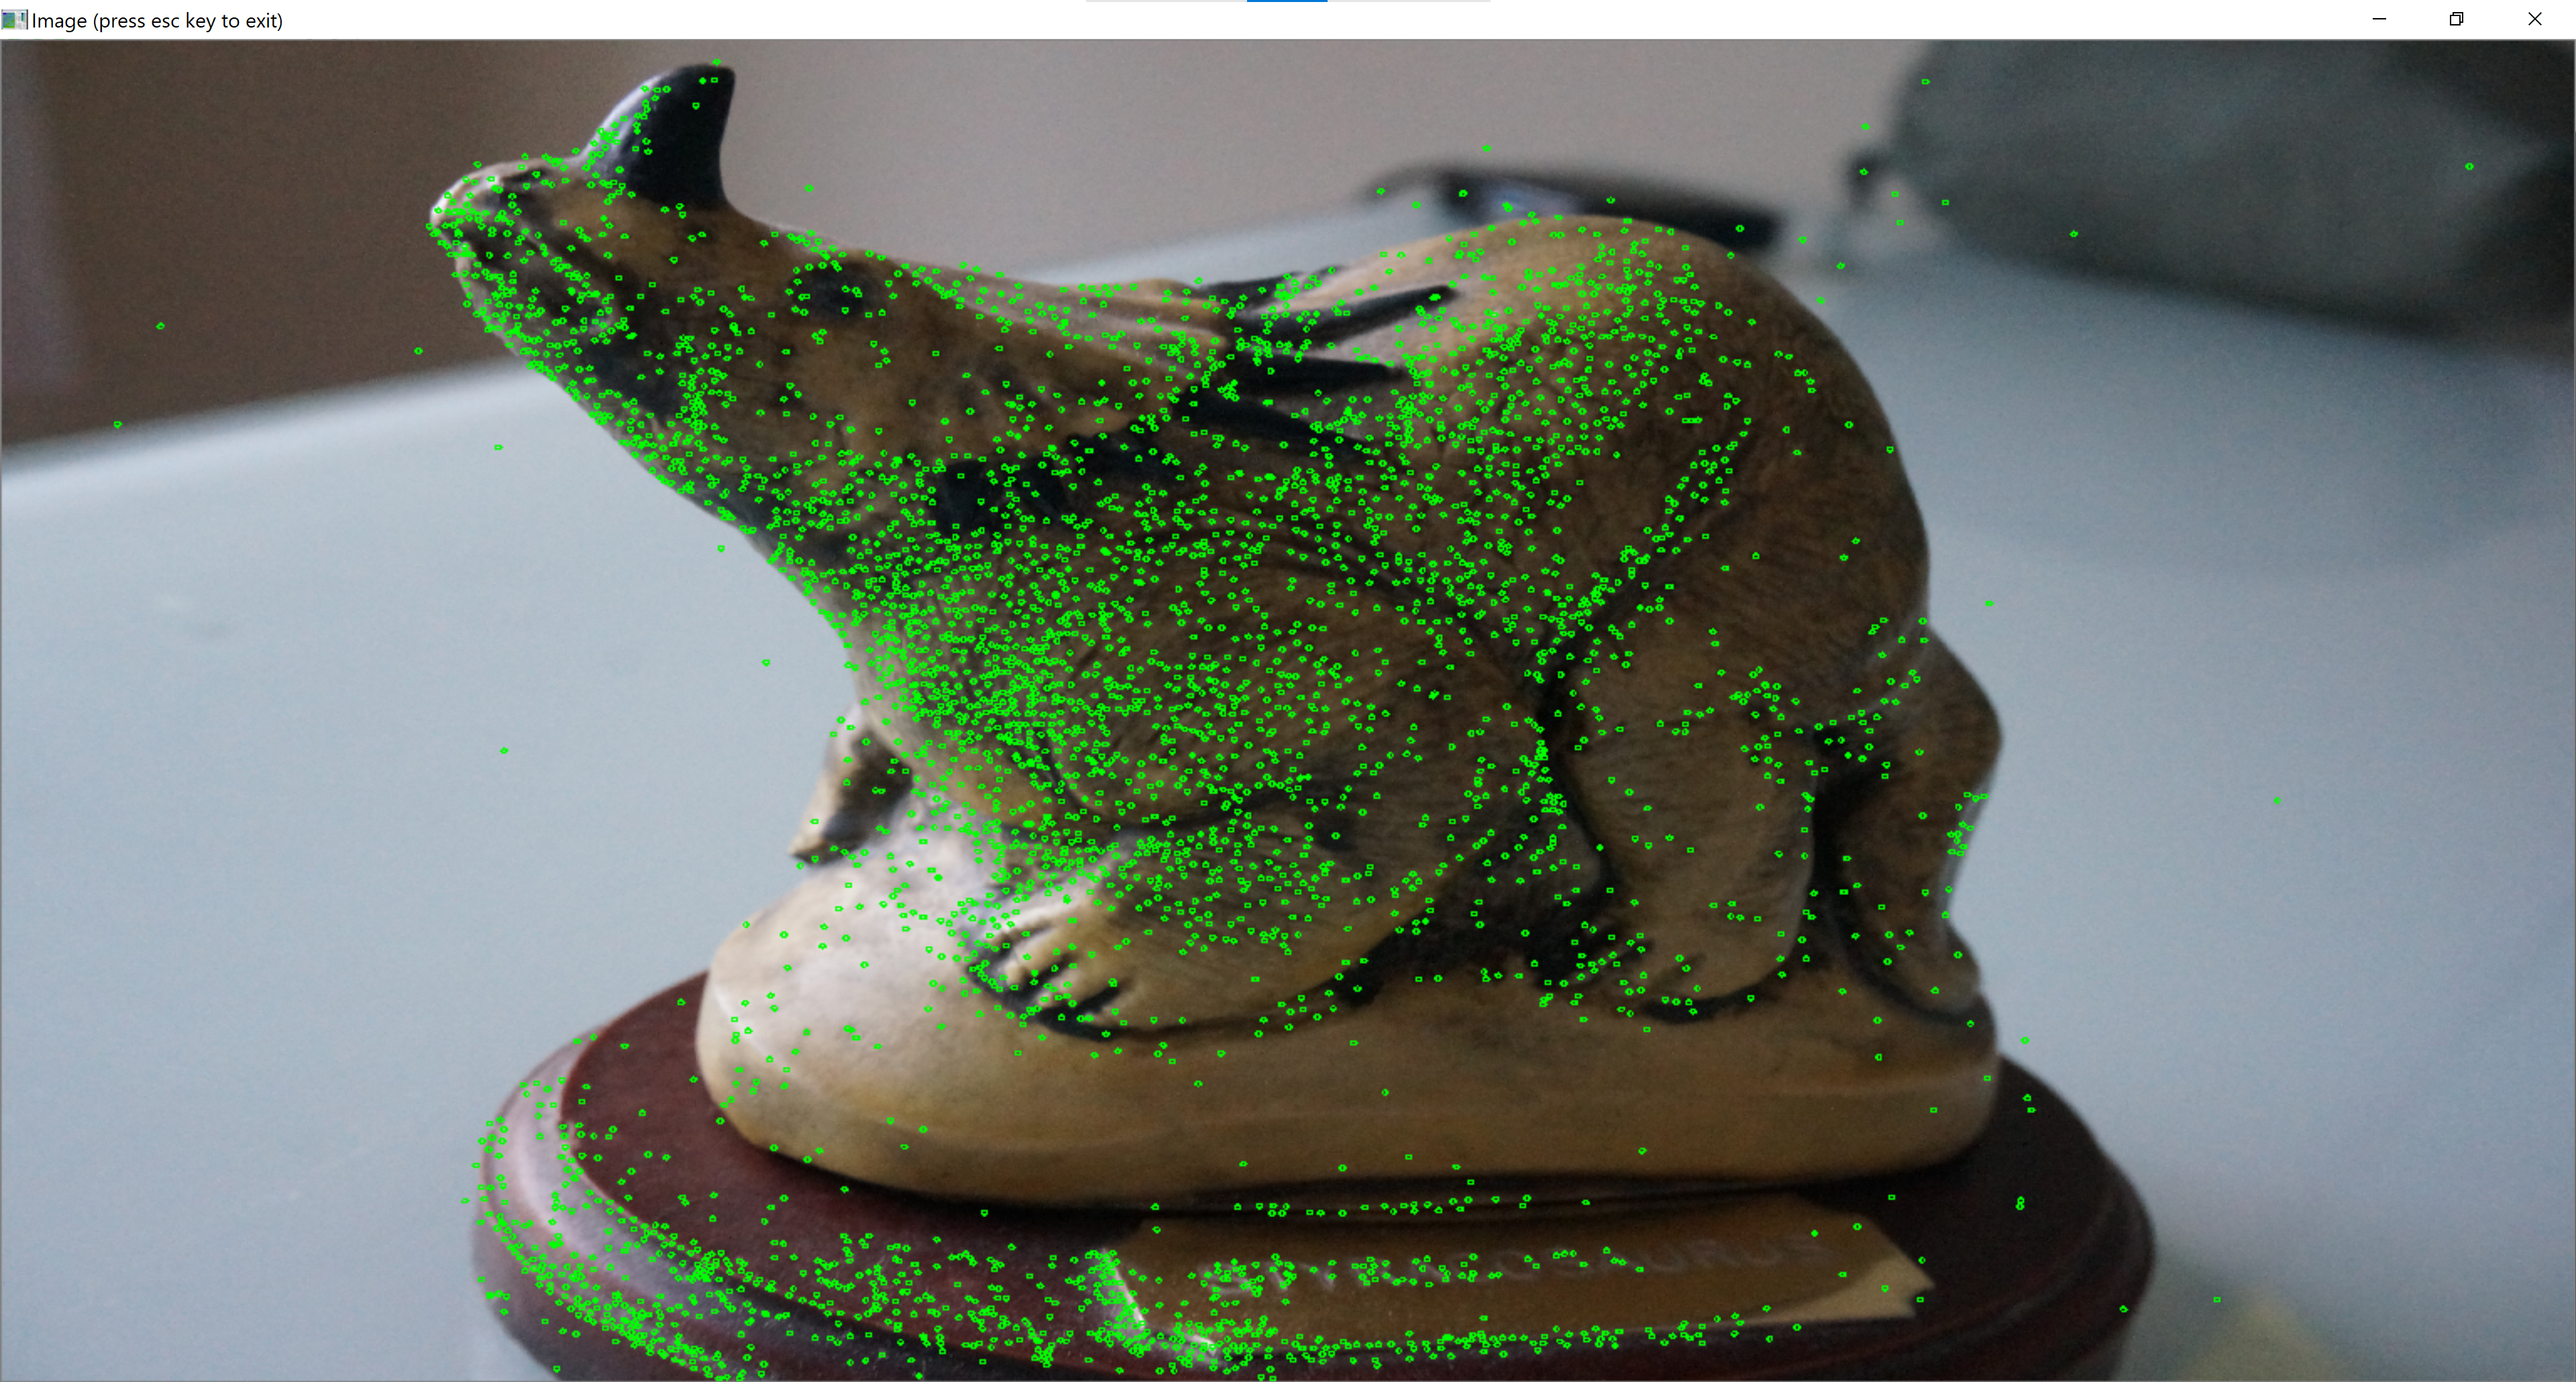
\includegraphics[width=\linewidth]{datas/helper/test_keyframe_dino.png}
    \end{subfigure}

    \begin{subfigure}{0.7\textwidth}
        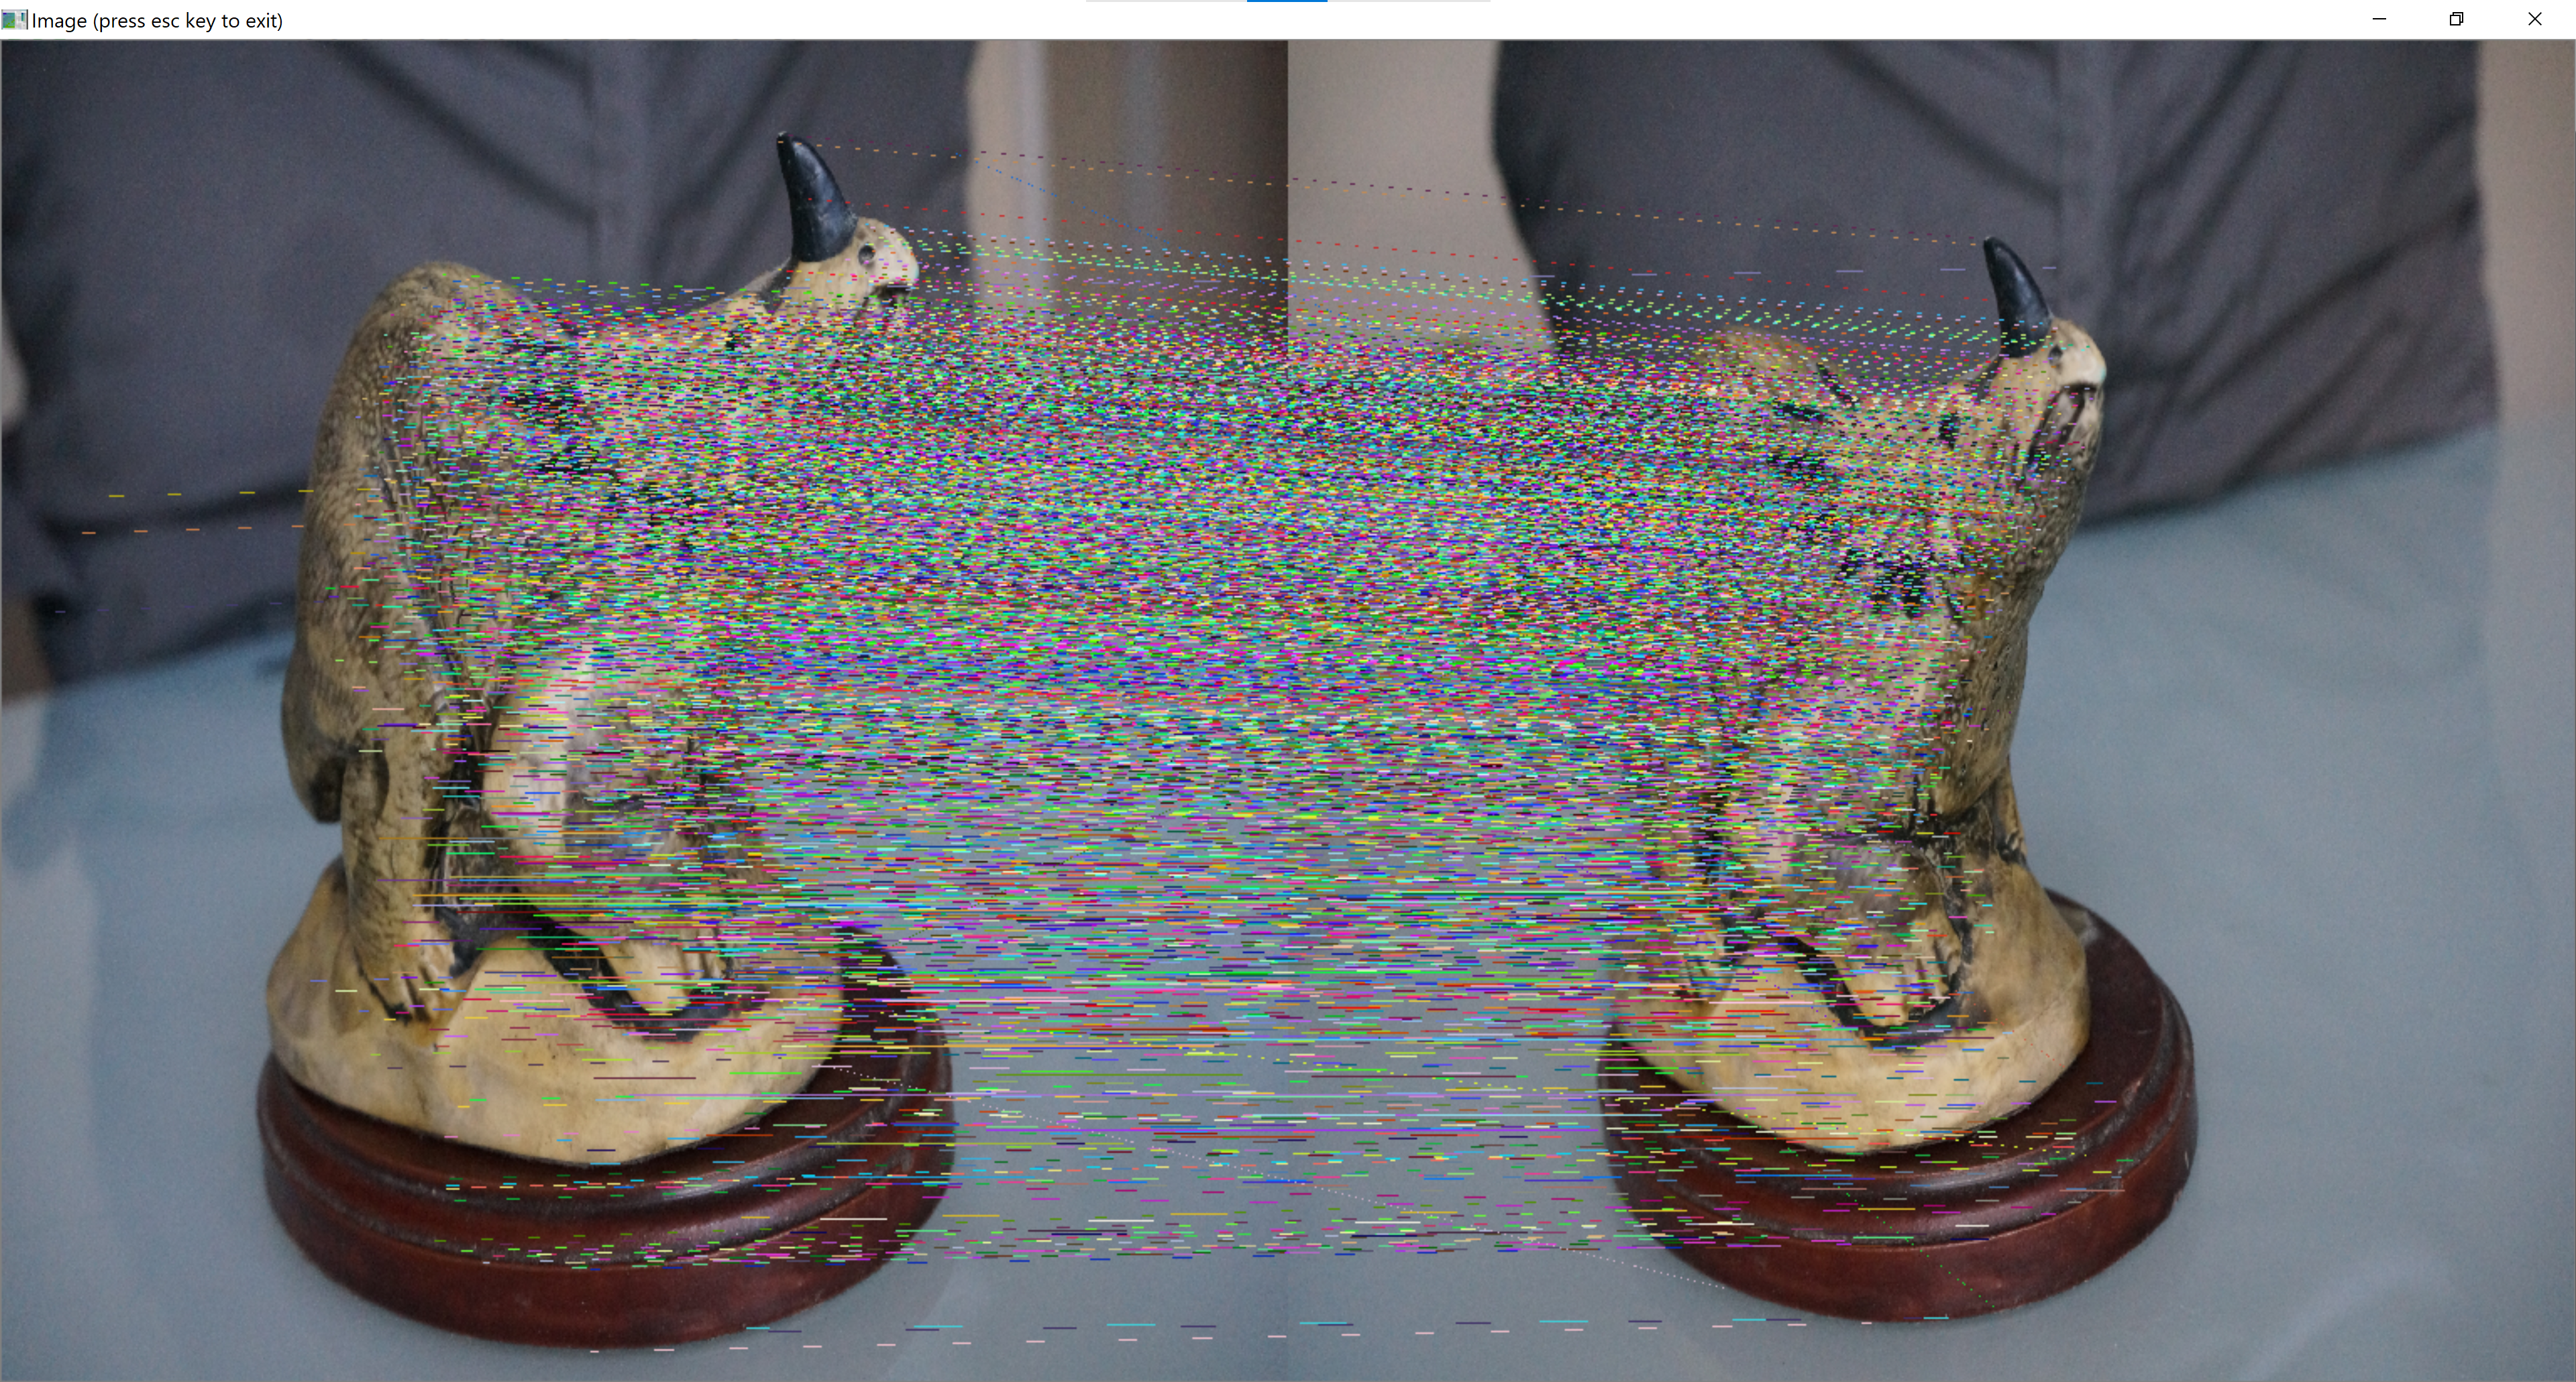
\includegraphics[width=\linewidth]{datas/helper/test_descriptors_dino.png}
    \end{subfigure}

    \begin{subfigure}{0.7\textwidth}
        \includegraphics[width=\linewidth]{datas/helper/test_pointcloud_dino.png}
    \end{subfigure}

    \caption{Résultats des tests pour le dataset Dinosaure}
    \label{fig:test_dino}
\end{figure}

\begin{figure}[ht]
    \centering
    \begin{subfigure}{0.7\textwidth}
        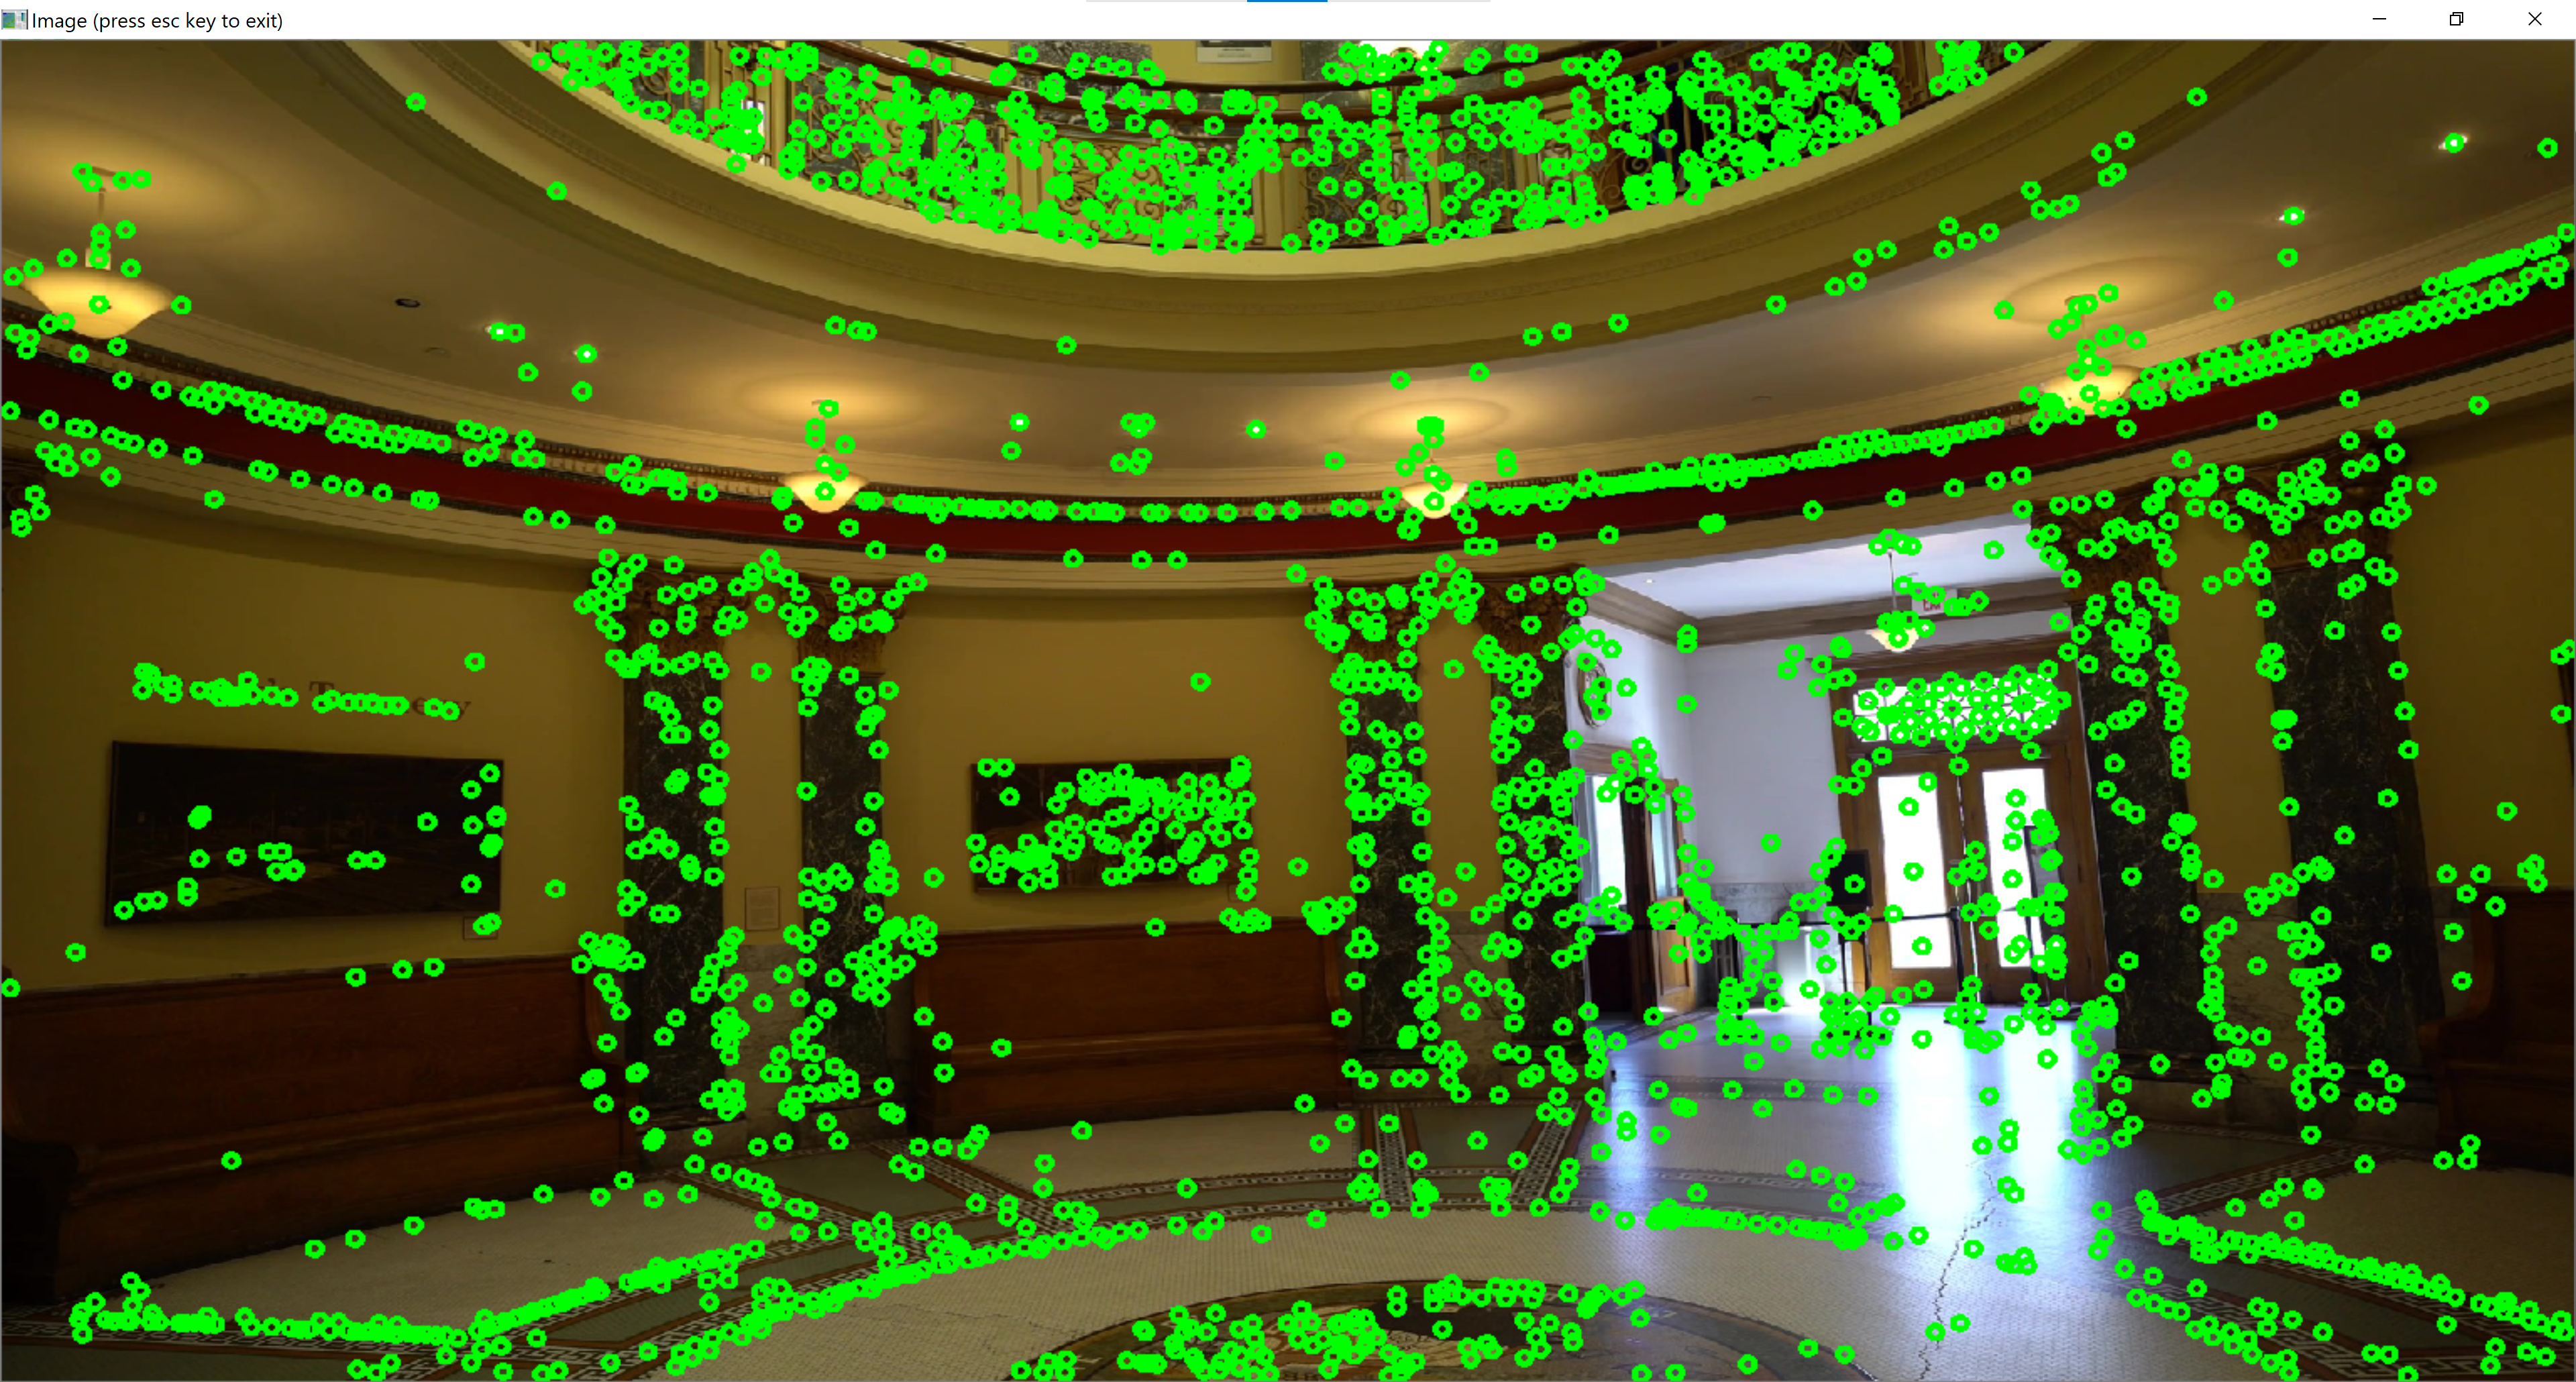
\includegraphics[width=\linewidth]{datas/helper/test_keyframe_museum.png}
    \end{subfigure}

    \begin{subfigure}{0.7\textwidth}
        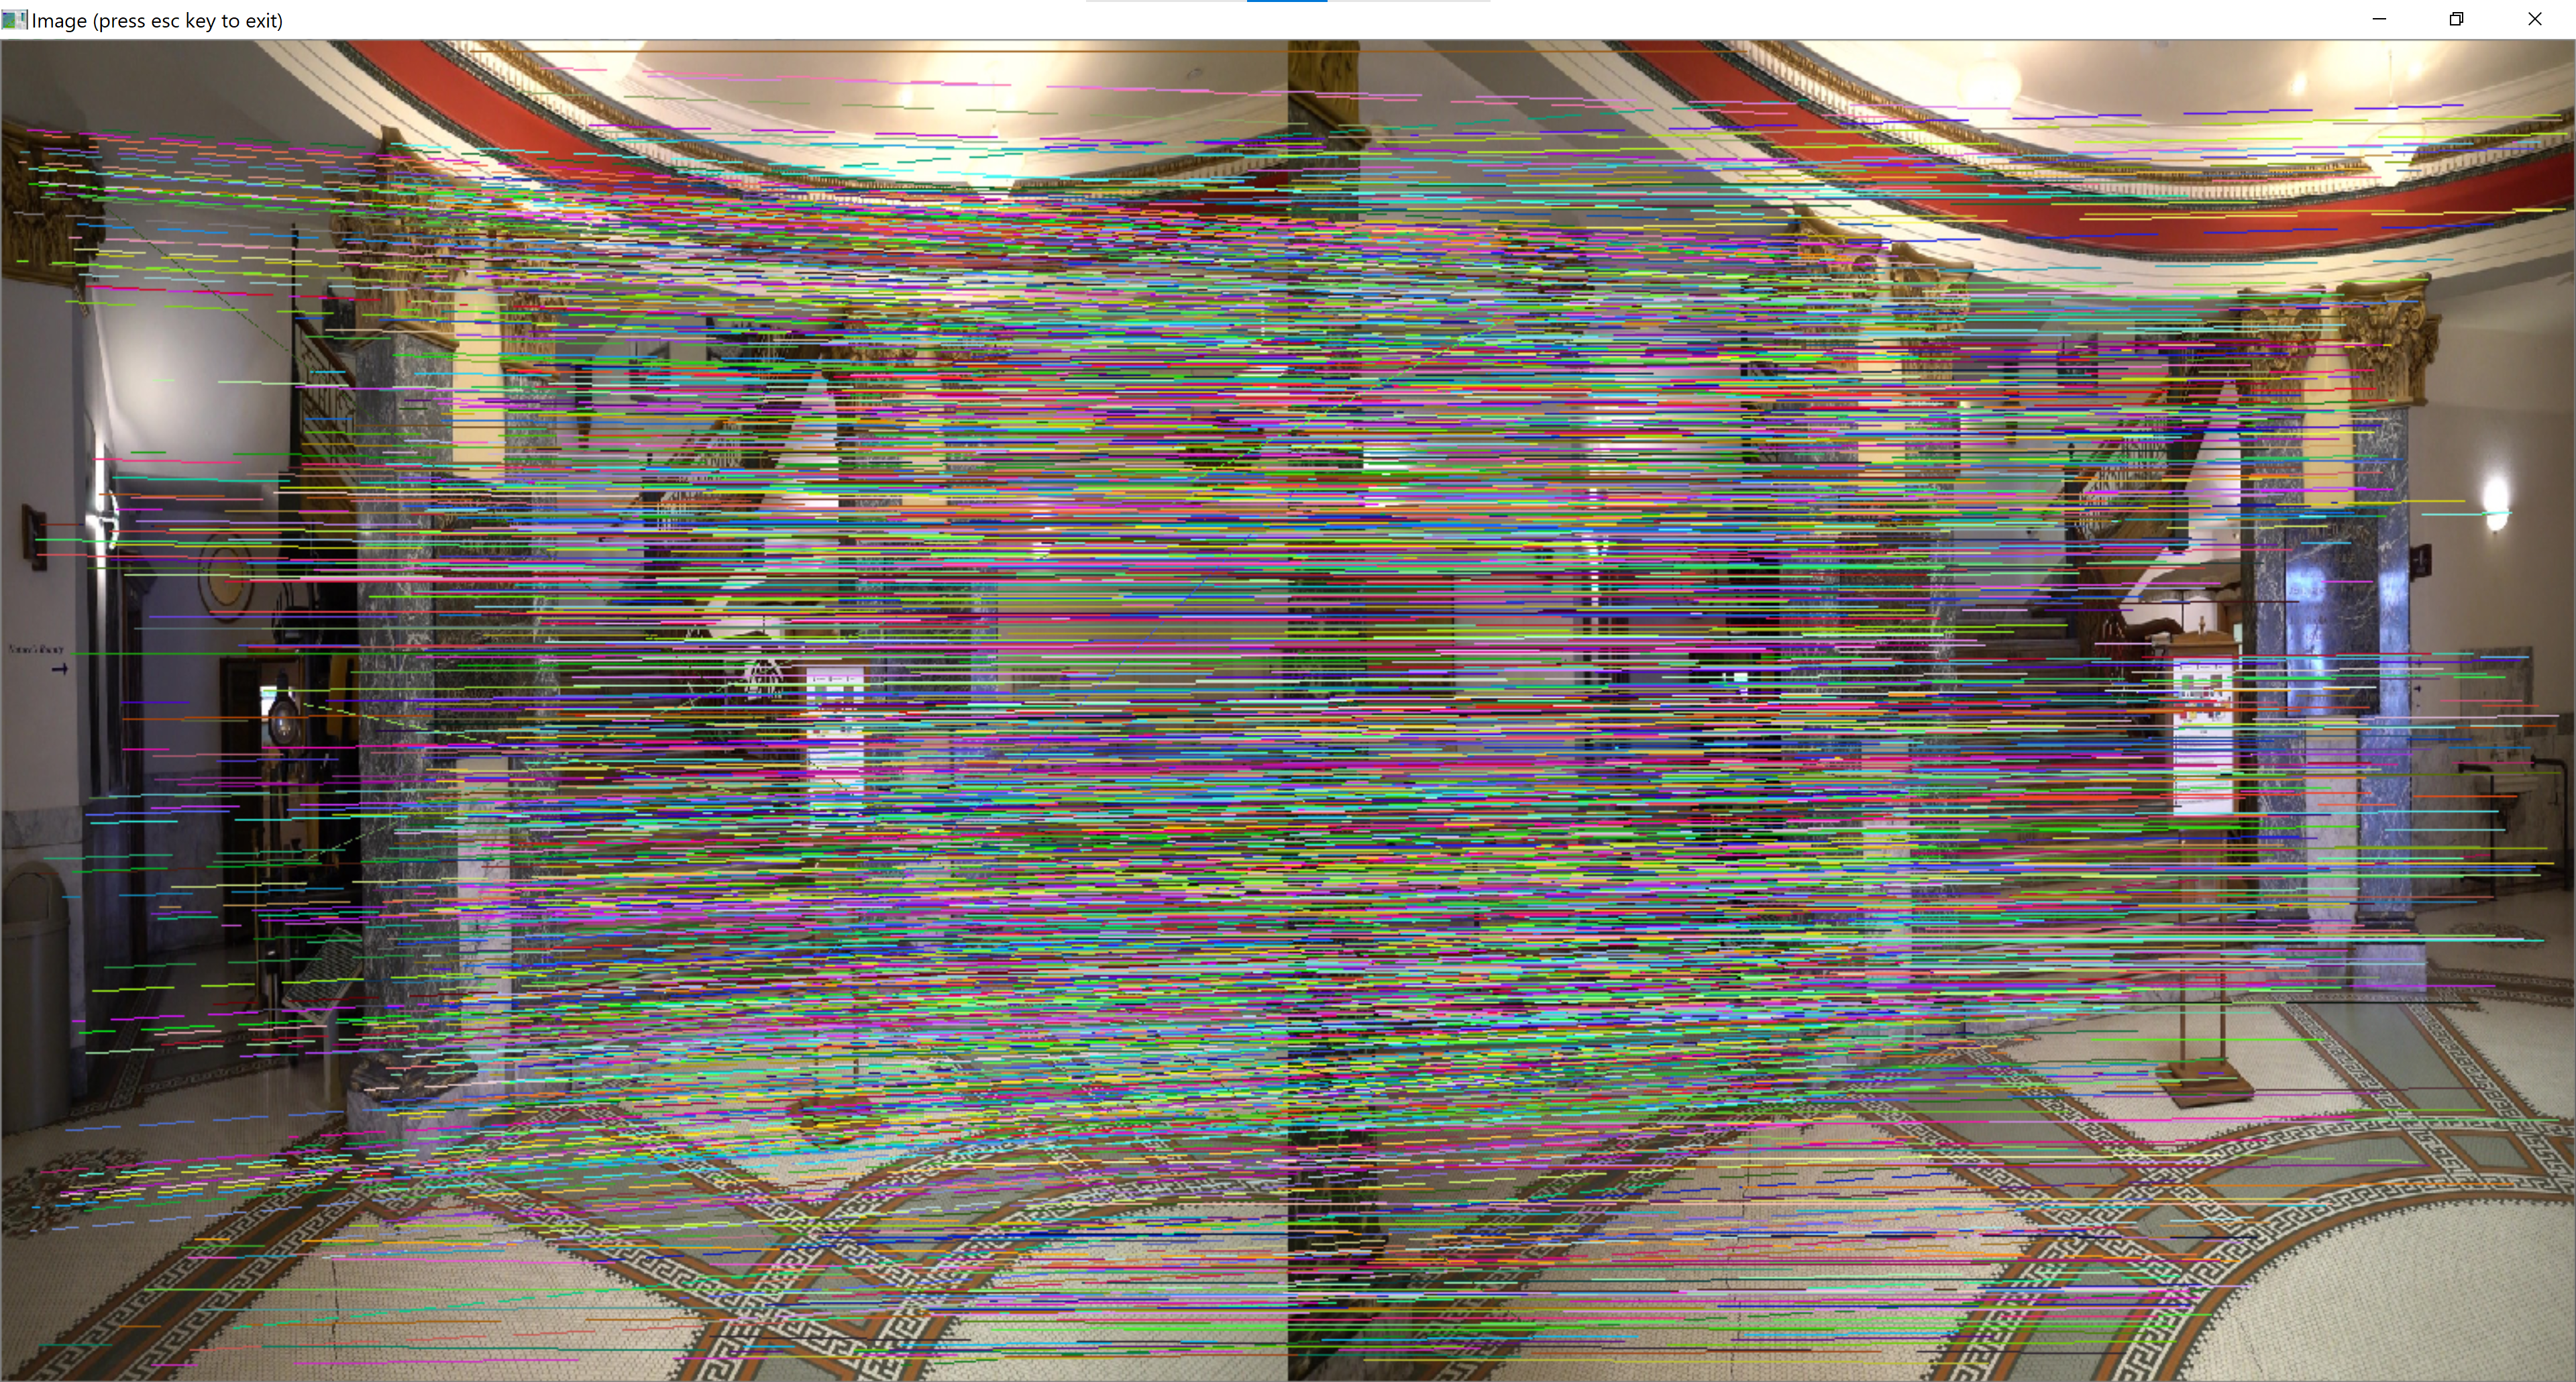
\includegraphics[width=\linewidth]{datas/helper/test_descriptors_museum.png}
    \end{subfigure}

    \begin{subfigure}{0.7\textwidth}
        \includegraphics[width=\linewidth]{datas/helper/test_pointcloud_museum.png}
    \end{subfigure}

    \caption{Résultats des tests pour le dataset Museum}
    \label{fig:test_museum}
\end{figure}

\end{document}